\documentclass{article}
\usepackage{iclr2026_conference,times}
% r48/B3 layout-only fix: tectonic (XeTeX) defaults to the TU encoding, for which
% no TUptm.fd exists, so `times` silently fell back to Latin Modern and dropped
% every bold/italic/small-caps shape (main.log: `TU/ptm/b/n' undefined, ...).
% Loading T1 restores the Times family required by the ICLR template together
% with \textbf/\emph/\textsc.  Zero prose, number, or citation change.
\usepackage[T1]{fontenc}
\usepackage{amsmath,amssymb,amsthm,booktabs,float,graphicx,microtype,multirow}
\newtheorem{theorem}{Theorem}
\newtheorem{corollary}[theorem]{Corollary}
\newtheorem{definition}[theorem]{Definition}
\newtheorem{assumption}[theorem]{Assumption}
\usepackage{url}
\usepackage{hyperref}
% r58 layout-only: hyperref's default link border (/Border[0 0 1]) is painted by
% poppler, so every \citep printed inside a green frame and every \ref inside a
% red one (verified at 300 dpi on the previous face: 3227 saturated green and 296
% red pixels on page 1 alone, frames clipping glyph descenders).  hidelinks drops
% the borders without recoloring any text.  No prose, number or citation change.
\hypersetup{hidelinks}
% R106 step 4 / human 23:42: byte-identical deterministic build.
% Build with tectonic (XeTeX) + fixed SOURCE_DATE_EPOCH; this is the only
% supported build entrypoint (see build/build_deterministic.sh) and yields
% identical SHA-256 across independent runs on the same source tree.
\newcommand{\method}{\textsc{SparseForge}}
\newcommand{\taskavg}{\textsc{Avg}-9}
\definecolor{sfblue}{HTML}{0072B2}
\definecolor{sforange}{HTML}{E69F00}

% R255 Route-C: the concise form keeps the negative result legible in the ICLR
% title block and removes an unsupported mechanism-level title claim.
% R93/G1: the previous title asserted "Below the Detection Floor" at title level,
% which the C1 self-check ruled an overclaim while the body disclaims it; a title
% that claims what the body denies is itself a fatal inconsistency.  The title now
% states the measured quantity (0.118 pp) and the reference scale it is compared
% against, with no normative detection-floor claim.
% R93/G1 line-break placement (typography only, word sequence verbatim):
% measured in the \LARGE\sc title font against \textwidth=397.49pt, the two
% breaks specified in the instruction overflow ("...Compression of"=411.79pt,
% "Cross-Support ... Sparsification ---"=429.92pt), which made TeX wrap them and
% print an orphan "OF" line plus a hyphenated "SPARSIFICA-/TION".  These five
% breaks all fit (275.30 / 325.05 / 237.04 / 349.48 / 372.05pt), keep the em dash
% at the title/subtitle boundary, and hyphenate nothing.
\title{SparseForge: Recovery-Induced\\ Compression of Cross-Support Spread\\ in 2:4 LLM Sparsification ---\\ A Registered Negative Result at 0.118 pp\\ Below the Harness's Sampling-Noise Scale}
\author{Anonymous Authors}

% R177/B2 0-GPU layout reclaim (round 45): typography metrics only, zero semantic change.
\emergencystretch=1.5em
\setlength{\itemsep}{1pt}
\setlength{\textfloatsep}{8pt plus 2pt minus 2pt}
\setlength{\floatsep}{8pt plus 2pt minus 2pt}
\setlength{\abovedisplayskip}{5pt plus 1pt minus 2pt}
\setlength{\belowdisplayskip}{5pt plus 1pt minus 2pt}

\begin{document}
\maketitle

\begin{abstract}
Hardware-supported semi-structured sparsity can accelerate large language models, but exact $2{:}4$ support selection is locally coupled and post-training recovery adds substantial cost. We report a negative result about what remains distinguishable after that recovery. Applying the same $625$M-token joint sparse-weight and rank-16 SLoRB recovery to three registered fixed supports---ALPS, ELSA-4096, and ProxSparse---compresses their cross-support \taskavg{} range from $2.675$\,pp to $0.118$\,pp. The recovered range is a scale far below the $0.52$\,pp per-checkpoint binomial-SE of this harness. That $0.52$\,pp is a single-checkpoint eval-sampling scale; pairwise per-item predictions were not retained for the three registered endpoints, so the joint uncertainty of the post-recovery range is not identifiable from the registered data, and we claim no pairwise or joint resolution limit. The transferable caution is that support- or mask-selection claims at this scale require paired per-item analysis that was not available here. The curvature score, soft-to-hard annealing schedule, and rank-16 SLoRB branch are therefore pipeline background rather than isolated explanations: these components have never been isolated under matched budgets, and none of the reported gains can be attributed to one component. As supporting context, the archived $5$B checkpoint measures $58.47$ \taskavg{} only with its SLoRB branch live; no folded exact-$2{:}4$ export or pre/post-export quality measurement exists. Because the training corpus provenance of this archived checkpoint is unavailable (the manifest lives on the unreachable archive host with the checkpoint; Appendix~\ref{app:implementation}), recovery-corpus interpretability is limited accordingly.
\end{abstract}

\section{Introduction}
Semi-structured sparsity is one of the few compression regimes that combines substantial parameter removal with native accelerator support. In particular, NVIDIA sparse Tensor Cores execute exact $2{:}4$ patterns, retaining two weights in every group of four~\citep{nvidia2020ampere}. The same constraint that makes deployment efficient also couples pruning decisions: each candidate competes locally, and a mistaken hard selection cannot be repaired without changing the support.

A basic empirical question is surprisingly absent from this literature: if several native supports are recovered under an \emph{identical} token budget and recipe, does cross-support spread persist, or does recovery compress it? Prior work compares methods against each other but does not label multiple supports per method and re-measure them after one fixed recovery run. This paper makes that archived measurement the load-bearing contribution; the SparseForge pipeline below is background context, not a validated mechanism.

Calibration-only methods such as Wanda and SparseGPT~\citep{sun2023wanda,frantar2023sparsegpt} are inexpensive, while retraining-based AST and CAST~\citep{huang2025ast,huang2025cast} recover more quality at larger token budgets. This leaves a practical question: can a recovery run spend its tokens on improving the structured support itself, rather than merely adapting weights to an early hard mask?

As pipeline background, \method{} (Figure~\ref{fig:pipeline}) maintains a continuous mask and alternates task/distillation updates of the sparse base weights and rank-16 SLoRB branch with periodic curvature-score mask updates. A soft-to-hard schedule then moves the mask toward an exact $2{:}4$ pattern. This describes the archived training pipeline rather than an isolated causal mechanism: the reported checkpoint keeps the SLoRB branch live, and folding it into a deployable exact-$2{:}4$ export is a registered future step (Appendix~\ref{app:implementation}), not an executed result. These three components have never been isolated under matched budgets; none of the reported gains can be attributed to any single mechanism.

The load-bearing result is instead the recovery-compression comparison in Table~\ref{tab:recovery-compression}. Before recovery, the three registered supports span $2.675$\,pp in \taskavg{}; after the same $625$M-token recovery, they span only $0.118$\,pp, well below the harness's per-checkpoint binomial-SE sampling-noise scale (eval-noise only; not a pairwise or joint resolution limit, because paired per-item predictions were not retained). The $0.52$\,pp term is a marginal single-checkpoint standard error, not a threshold, detection floor, or equivalence margin; whether the three supports are separable at that scale is untested given that paired per-item statistics were not retained. The archived $5$B comparison in Table~\ref{tab:unified} and Figure~\ref{fig:checkpoint} remains supporting context, not mechanism evidence. We make three contributions:
\begin{minipage}{\linewidth}
\begin{itemize}
  \item an archived descriptive observation that identical recovery compresses cross-support \taskavg{} spread from $2.675$ to $0.118$\,pp, a point-estimate range far below the harness's per-checkpoint binomial-SE eval-sampling scale (paired or joint significance not testable because per-item predictions were not retained);
  \item a measurement-caution: paired per-item analysis and joint bounds are required before the supports can be compared at this scale, which this study did not register; and
  \item a unified local evaluation that separates fixed-support recovery from an archived branch-active checkpoint and preserves its corpus and export boundaries.
\end{itemize}
\end{minipage}

\begin{figure}[tb]
  \centering
  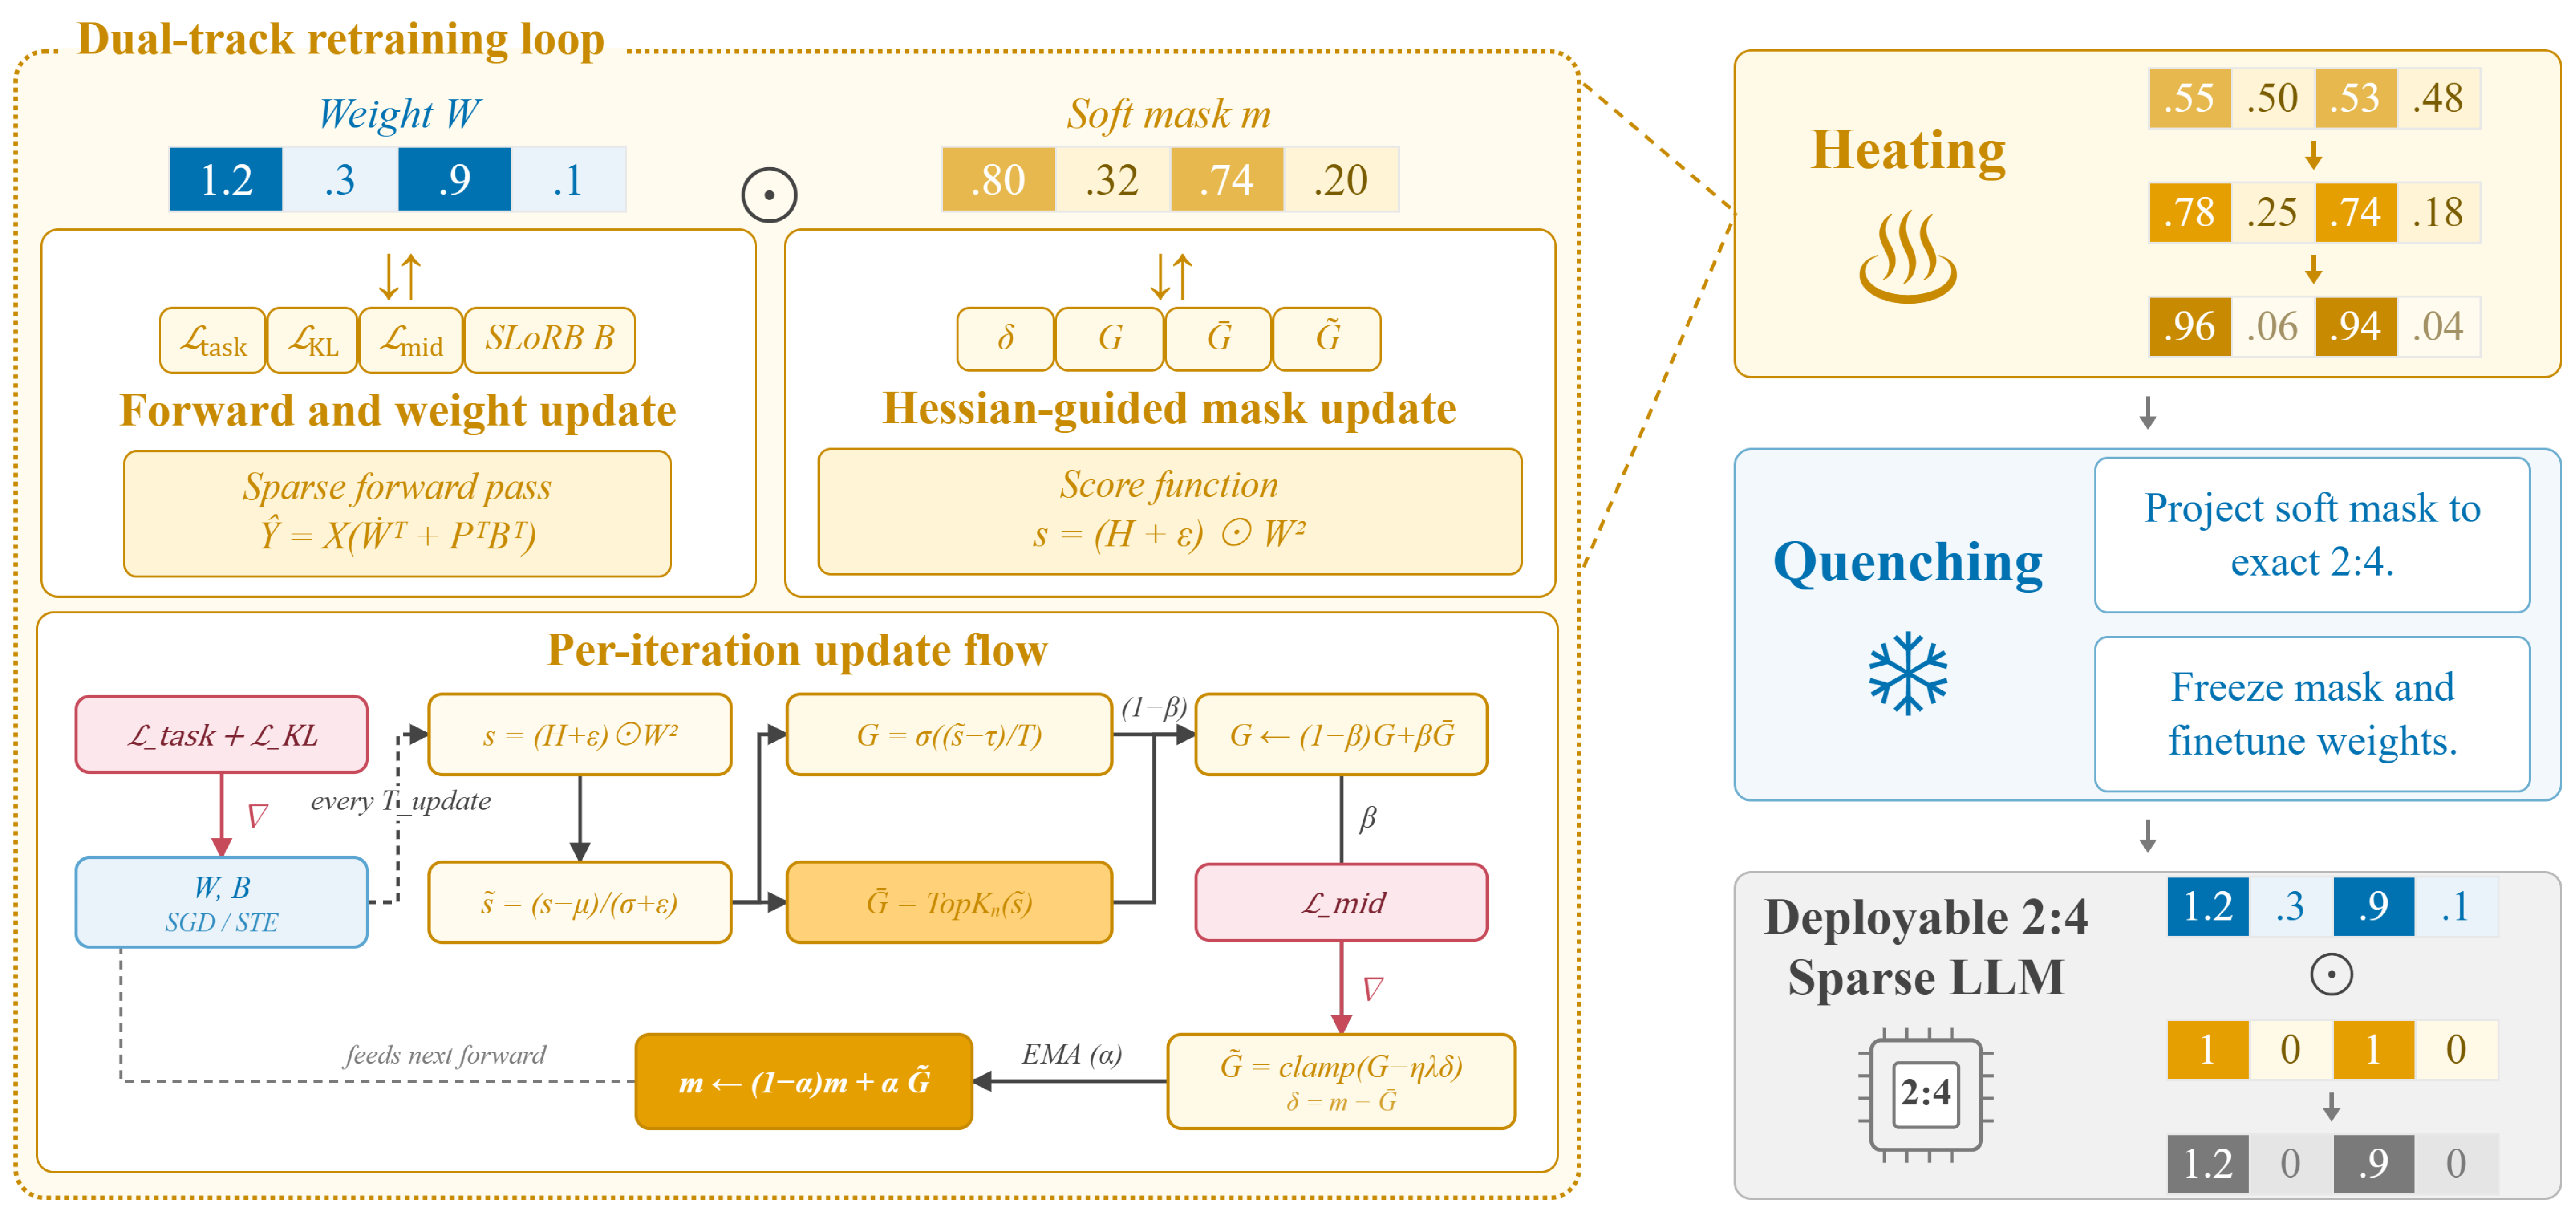
\includegraphics[width=0.98\textwidth]{images/SparseForge_pipeline.pdf}
  \caption{\textbf{SparseForge pipeline background.} The weight track updates sparse base weights $W$ and rank-16 SLoRB parameter $B$ using task and distillation losses. A separate periodic mask track computes curvature-based importance, constructs a soft group gate, and anneals it toward an exact $2{:}4$ target. Quenching freezes the support; the dashed fold/re-projection step depicted as the export arrow is the planned branch fold and re-projection, which is shown for completeness and is \emph{not executed} by the frozen finalizer---this paper reports only the branch-active training-state checkpoint upstream of that boundary. The regularizer $\mathcal{L}_{\mathrm{mid}}$ affects the dedicated mask update, not the weight-loss autograd path. The diagram describes the pipeline and is not evidence that any component causes the reported result. The in-figure annotations are set below body-text size so that the weight track, the mask track, and quenching fit one column width; the key symbolic annotations ($s$, $G$, $m$, $\widehat Y$) follow the macro naming of Sec.~\ref{sec:method}.}
  \label{fig:pipeline}
\end{figure}

\section{Related Work}
\paragraph{One-shot and calibration-scale pruning.}
Magnitude pruning and second-order criteria established the basic importance-estimation view~\citep{han2015magnitude,lecun1990obd,hassibi1993obs}. For LLMs, SparseGPT uses approximate second-order information and Wanda combines weights with activation statistics~\citep{frantar2023sparsegpt,sun2023wanda}. ALPS performs layerwise constrained reconstruction~\citep{meng2024alps}; ELSA and ProxSparse optimize semi-structured supports or parameters at calibration scale~\citep{lee2026elsa,liu2025proxsparse}. These approaches avoid a large recovery corpus, but their support decisions remain consequential under exact local structure.

\paragraph{Semi-structured sparse training.}
MaskLLM learns discrete $N{:}M$ masks with a large corpus, so its mask is trained rather than frozen from a calibration decision~\citep{fang2024maskllm}. AST anneals dense weights toward $2{:}4$ and uses SLoRB for recovery~\citep{huang2025ast}; CAST uses a continuous differentiable relaxation~\citep{huang2025cast}. To our knowledge none of these works report the post-recovery comparison of \emph{multiple} native supports: none fixes and labels several supports, applies an identical recovery run to each, and measures whether cross-support spread compresses below the eval-sampling scale. \method{} shares the aim of learnable structure with this literature, but the load-bearing result in this paper is exactly that archived, previously unreported cross-support measurement---not a novel algorithmic advantage. Like MaskLLM, AST, and CAST, the SparseForge mask trajectory itself was never isolated under matched budgets, so this work contributes measurement evidence and an honest boundary on what an archived training pipeline can and cannot establish, rather than a new mechanism claim.

\section{Pipeline Rationale (Background)}
In a group of four weights, one incorrect survivor necessarily excludes another candidate. A one-shot score can therefore select a poor subspace before recovery begins. Keeping the mask soft allows repeated evidence to reverse early rankings, but a soft gate is not deployable. The central problem is consequently a constrained transition: preserve exploration early, inject exact group structure progressively, and minimize the final soft-to-hard projection gap.

Curvature gives a local survival signal. For a weight $w_i$ near a pretrained solution,
\begin{equation}
\Delta L_i \approx -\frac{\partial L}{\partial w_i}w_i + \frac{1}{2}\frac{\partial^2 L}{\partial w_i^2}w_i^2.
\end{equation}
When the first-order term is small, magnitude alone misses the loss curvature associated with deletion. Optimal Brain Damage motivates second-order importance via a \emph{diagonal} Hessian proxy~\citep{lecun1990obd}, while Optimal Brain Surgeon and WoodFisher go beyond the diagonal precisely because cross-term and inverse-curvature effects matter under exact structure~\citep{hassibi1993obs,singh2020woodfisher}: for $N{:}M$ groups the deleting mask couples coordinates within a group, so the diagonal term is only a first-order faithful ranking signal, not a certificate. \method{} therefore uses the diagonal curvature score to rank \emph{candidates} within each structured group (the cheap sufficient signal for which column of a $2{:}4$ group to drop) and makes no stronger approximation claim than OBD; annealing, not the curvature proxy alone, is what introduces the final support gradually. Throughout this paper we use ``match'' in the sense of numerical equivalence within stated sampling error, not of verified behavioral equivalence between checkpoints; per-item agreement between SparseForge and AST has not been established in this workspace.

\section{Training Pipeline}\label{sec:method}
For reproducibility, we describe the archived training pipeline that produced the registered endpoints; the description is background and does not isolate component effects. Let a linear layer be $Z=XW^\top$, with $W\in\mathbb{R}^{D\times C}$, and let $m\in[0,1]^{D\times C}$ be a soft mask. The effective sparse weight is $\widetilde W=m\odot W$. For a fixed projection $P$ and learnable rank-16 SLoRB matrix $B$, the reported strong configuration computes
\begin{equation}
\widehat Y=X(\widetilde W^\top+P^\top B^\top).
\end{equation}

\subsection{Reported Weight and Mask Tracks}
The weight track minimizes next-token cross-entropy plus teacher-to-student KL divergence,
\begin{equation}
\mathcal{L}_{W,B}=\lambda_{\mathrm{task}}\mathcal{L}_{\mathrm{task}}+\lambda_{\mathrm{KL}}\mathcal{L}_{\mathrm{KL}},
\end{equation}
updating both $W$ and $B$. The mask is a non-autograd buffer with a dedicated periodic rule. This separation permits frequent weight adaptation while avoiding a noisy mask decision at every minibatch. It also makes the method explicitly joint: the support, sparse base weights, and recovery branch all change during the strong run.

\subsection{Curvature-Score Background}
For each layer, we estimate diagonal curvature with a Hutchinson-style probe~\citep{hutchinson1990trace} and maintain an exponential moving average. The survival score is
\begin{equation}
s=\Bigl(\max(H,0)+\epsilon\Bigr)\odot W^2.
\end{equation}
where $H$ is the Hutchinson-estimated diagonal and the element-wise clamp at zero prevents sign reversals from mis-estimated negative diagonal entries from re-ordering the within-group ranking.
After layer-wise standardization, each non-overlapping group $g$ of $M$ entries forms a soft gate and a structured target,
\begin{equation}
G_g=\sigma\!\left((\widetilde s_g-\tau_g)/T\right),\qquad
\bar G_g=\operatorname{TopK}_{N}(\widetilde s_g),
\end{equation}
where $\tau_g$ is the midpoint between the $N$th- and $(N{+}1)$th-largest standardized scores; the frozen implementation instead uses the $N$th-largest score itself, so the $N$th-ranked candidate sits exactly at threshold rather than strictly above it (Appendix~\ref{app:implementation}). $T$ controls decisiveness without immediately committing to a binary support.

\subsection{Soft-to-Hard Schedule and Deployment Boundary}
We progressively mix the exploratory gate with its feasible target,
\begin{equation}
G\leftarrow(1-\beta)G+\beta\bar G,
\end{equation}
while decreasing $T$ and ramping a mild binary-target penalty $\mathcal{L}_{\mathrm{mid}}=\lVert m-\bar G\rVert_F^2/(2|m|)$. The dedicated mask update moves a clipped gate toward $\bar G$ and then applies an exponential moving average. Near the end, an interpolation $m_{\mathrm{eff}}=xm+(1-x)\mathrm{1}[m>\theta]$ moves from the soft mask to the binary mask. The scheduled construction would then fold the branch into the weights and re-apply exact $2{:}4$ projection. This is a scheduled construction, not a theoretical convergence guarantee. In the frozen implementation the schedule stops at the branch-active checkpoint: the branch fold and exact $2{:}4$ re-projection are specified but not executed (Appendix~\ref{app:implementation}), so every downstream number is a training-state measurement.
All hyperparameters of the reported strong configuration are collected in
Table~\ref{tab:hyperparams} (Appendix~\ref{app:implementation}).

\subsection{Notation}
Throughout, SLoRB denotes the \textbf{S}parse-\textbf{L}ow-\textbf{R}ank
\textbf{B}ranch~\citep{huang2025ast}: a fixed projection $P$ and learnable
rank-16 matrix $B$ whose product $B P$ participates in every training-state
evaluation; the algebraic fold of $B P$ into the weights at quenching time is
specified but not implemented by the frozen finalizer (Appendix~\ref{app:implementation}),
and is registered as future export work.

\section{Experiments}
\subsection{Setup}
The primary study uses LLaMA-2-7B~\citep{touvron2023llama2} at exact $2{:}4$ sparsity. The main checkpoint performs $5$B-token recovery; its training corpus provenance is unavailable (the archived manifest lives with the checkpoint on a host unreachable from this workspace; Appendix~\ref{app:implementation}), so the corpus is not named in this paper. We evaluate zero-shot plain accuracy with lm-evaluation-harness~\citep{biderman2024lmeval} on BoolQ, RTE, HellaSwag, WinoGrande, ARC-Easy, ARC-Challenge, OpenBookQA, RACE, and PIQA~\citep{clark2019boolq,wang2019superglue,zellers2019hellaswag,sakaguchi2021winogrande,clark2018arc,mihaylov2018openbookqa,lai2017race,bisk2020piqa}. \taskavg{} is the task-equally-weighted nine-task aggregate (unweighted mean of the nine per-task accuracies; each task contributes $1/9$ regardless of its dev-set size). We also report WikiText-2 perplexity. Every reported evaluation, including the headline row, is of the branch-active training-state checkpoint (SLoRB branch live at inference); no folded or re-projected export exists, and export-equivalence is prospective (Appendix~\ref{app:implementation}).

Table~\ref{tab:unified} separates native calibration/short-optimization checkpoints from fixed-support recovery. Each recovery row fixes the named support and jointly trains sparse base weights plus zero-initialized rank-16 SLoRB for $624{,}951{,}296$ tokens (reported as $625$M). The public AST export and the archived \method{} checkpoint are evaluated locally; the AST publication does not disclose its own recovery-token budget or recovery corpus, so the AST row is a quality anchor rather than a matched-budget control. The 5B comparison is a single-checkpoint point estimate; historical repeated runs are confined to Appendix~\ref{app:history}. For the pending matched-budget arm we tokenized a $1.366$B-token Dolmino-mix-1124 recovery stream locally, and its validation split is an $8192$-token prefix of that same training stream (\texttt{val = train[:8192]}); it serves only as an early-step sanity signal for perplexity stability, not as an independent held-out set, so no generalization claim is drawn from it.

\begin{table*}[t]
\centering
\caption{Unified LLaMA-2-7B evaluation at exact $2{:}4$ sparsity. Task cells are local plain-accuracy percentages; PPL is WikiText-2. Wanda, SparseGPT, ALPS, and ELSA are three-seed means. Recovery rows are not native checkpoints. The $625$M \method{} fixed-support matched-budget arm\protect\footnotemark[1] and the recovery token budget and corpus of the public AST checkpoint are registered gaps; the AST row is a quality anchor with under-reported recovery-budget provenance, not a matched-budget control. This aggregate supports the archived AST comparison; Appendix~\ref{app:dispersion}, Table~\ref{tab:dispersion} reports baseline dispersion. Task abbreviations: BQ = BoolQ, Hella. = HellaSwag, Wino. = WinoGrande, ARC-e/c = ARC-Easy/Challenge, OBQA = OpenBookQA. The \method{} row is a branch-active training-state checkpoint (SLoRB live at inference); a folded exact-$2{:}4$ export has never been produced or measured (Appendix~\ref{app:implementation}, EXT-M3). The \method{} row is additionally a $5$B-token recovery checkpoint whose training-corpus provenance is unavailable (archived with the checkpoint; Appendix~\ref{app:implementation}); only the pending matched-budget arms use a locally tokenized Dolmino-mix-1124 stream.}
\label{tab:unified}
\setlength{\tabcolsep}{3pt}
% Final visual audit: the former 12-column body required 7pt \scriptsize.
% Split the metrics into two row-aligned panels so every registered cell remains
% in the main table at the template's readable 9pt \small size.  No scaling is
% used, and the method order/group rules are repeated to preserve comparison.
\renewcommand{\arraystretch}{1.0}
\small
\begin{tabular*}{\textwidth}{@{\extracolsep{\fill}}lrrrrr}
\multicolumn{6}{@{}l}{\textit{(a) Per-task accuracy: BoolQ through ARC-Easy}} \\
\toprule
Method & BQ & RTE & Hella. & Wino. & ARC-e \\
\midrule
Dense reference & 79.45 & 62.82 & 57.10 & 69.61 & 75.55 \\
\midrule
Wanda (3 seeds) & 68.08 & 53.07 & 41.45 & 61.64 & 61.73 \\
SparseGPT (3 seeds) & 70.72 & 55.96 & 45.03 & 64.98 & 63.23 \\
ALPS (3 seeds) & 67.65 & 54.87 & 46.36 & 65.30 & 64.60 \\
ELSA (4,096 steps; 3 seeds) & 69.79 & 58.72 & 50.95 & 66.19 & 67.33 \\
ProxSparse (official) & 68.53 & 56.68 & 47.94 & 63.61 & 64.31 \\
\midrule
ALPS mask + recovery (625M) & 69.72 & 62.45 & 52.60 & 67.09 & 69.53 \\
ELSA mask + recovery (625M) & 72.94 & 59.57 & 52.19 & 66.85 & 70.79 \\
ProxSparse mask + recovery (625M) & 71.96 & 61.73 & 52.12 & 66.61 & 70.37 \\
\midrule
AST official deployable & 74.50 & 65.34 & 54.71 & 68.19 & 73.36 \\
\method{} (archived corpus\footnotemark[2], 5B) & 78.47 & 49.82 & 54.65 & 69.85 & 76.39 \\
\bottomrule
\end{tabular*}
\vspace{4pt}

\begin{tabular*}{\textwidth}{@{\extracolsep{\fill}}lrrrrrr}
\multicolumn{7}{@{}l}{\textit{(b) Per-task accuracy: ARC-Challenge through PIQA, with aggregate and PPL}} \\
\toprule
Method & ARC-c & OBQA & RACE & PIQA & \taskavg & PPL \\
\midrule
Dense reference & 42.75 & 33.20 & 39.52 & 77.86 & 59.76 & 5.5637 \\
\midrule
Wanda (3 seeds) & 29.78 & 23.47 & 35.95 & 70.37 & 49.50 & 12.3911 \\
SparseGPT (3 seeds) & 32.39 & 25.20 & 37.51 & 71.82 & 51.87 & 10.0569 \\
ALPS (3 seeds) & 32.14 & 26.13 & 38.50 & 73.56 & 52.12 & 10.3270 \\
ELSA (4,096 steps; 3 seeds) & 35.07 & 28.47 & 39.46 & 75.37 & 54.59 & 7.9832 \\
ProxSparse (official) & 33.53 & 25.00 & 35.79 & 71.87 & 51.92 & 9.2992 \\
\midrule
ALPS mask + recovery (625M) & 35.58 & 28.00 & 40.96 & 76.44 & 55.82 & 7.1006 \\
ELSA mask + recovery (625M) & 36.52 & 28.60 & 39.81 & 76.17 & 55.94 & 7.1121 \\
ProxSparse mask + recovery (625M) & 36.18 & 28.00 & 39.90 & 76.28 & 55.91 & 7.1284 \\
\midrule
AST official deployable & 39.51 & 30.00 & 38.85 & 76.99 & 57.94 & 6.3430 \\
\method{} (archived corpus\footnotemark[2], 5B) & 43.86 & 35.20 & 41.63 & 76.33 & \textbf{58.47} & \textbf{6.2179} \\
\bottomrule
\end{tabular*}
\end{table*}
% MINOR-6 fix (r72 full-fix): the all-em-dash T1 row was dropped from
% Table~\ref{tab:unified}; this table note replaces it.  \stepcounter is needed
% because \footnotetext alone reuses the current (zero) counter value and printed
% an orphan footnote "0" on the previous face.
\stepcounter{footnote}\footnotetext{The 625M matched-budget arm is registered as a pending measurement.}
\stepcounter{footnote}\footnotetext{The recovery corpus of this archived 5B checkpoint is not named because its provenance is unverifiable in this workspace: the training manifest and checkpoint live on an unreachable archive host (Appendix~\ref{app:implementation}); the pending matched-budget arm tokenizes a locally controlled Dolmino-mix-1124 stream instead.}

Under this harness, the per-checkpoint binomial-SE of \taskavg{} is $0.52$\,pp (Appendix~\ref{app:sf-ast-stats}); this is a single-checkpoint eval-sampling scale only, not a detection floor for pairwise or joint claims. The $0.52$\,pp term is a pre-declared harness quantity: it is the binomial standard error computed from the standard lm-eval dev-set sizes $n_k$ listed with their tasks in Table~\ref{tab:loo} (derivation in Appendix~\ref{app:sf-ast-stats}), fixed by the harness protocol and independent of the archived spread endpoints, so the marginal-scale comparisons above are not derived from the measurements they bound.

\subsection{Recovery Compression as the Load-Bearing Result}
The three native supports in Table~\ref{tab:unified} span $2.675$\,pp in \taskavg{}. Applying the same $625$M-token joint sparse-weight and SLoRB recovery to each support narrows that range to $0.118$\,pp (Table~\ref{tab:recovery-compression}), far below the $0.52$\,pp per-checkpoint binomial-SE sampling-noise scale. This is an archived descriptive observation: the identical recovery improves every fixed-support endpoint, yet the residual cross-support range cannot be tested against a pairwise or joint significance level from the registered aggregate CSVs, because the per-item statistics needed for that test were not retained. It is therefore a historical endpoint fact, not a statistical negative result or equivalence claim.

Figure~\ref{fig:checkpoint} retains the archived $5$B comparison as supporting context. Its $+0.53$-point aggregate conceals strongly mixed task-level behavior: the gain is concentrated in BoolQ, ARC, OpenBookQA, and RACE, while RTE moves by $-15.52$ points against \method{}. The aggregate remains within sampling noise and is too small to support broad superiority. It also does not establish a matched-budget \method{} advantage because no valid $625$M-token \method{} endpoint exists in this protocol. Under validated provenance the per-task pattern could suggest a recovery-corpus composition effect, but that corpus is not verifiable in this workspace (Appendix~\ref{app:implementation}), so no corpus-composition attribution is claimed; the matched controls needed to separate these attributions remain pending (Sec.~\ref{sec:conclusion}).

\begin{figure}[t]
  \centering
  % r48/B3 layout-only: 0.7 shrank the 8pt tick/value labels to ~5.7pt effective.
  % Page budget is 5 of 9 main-text pages, so widen for legibility.
  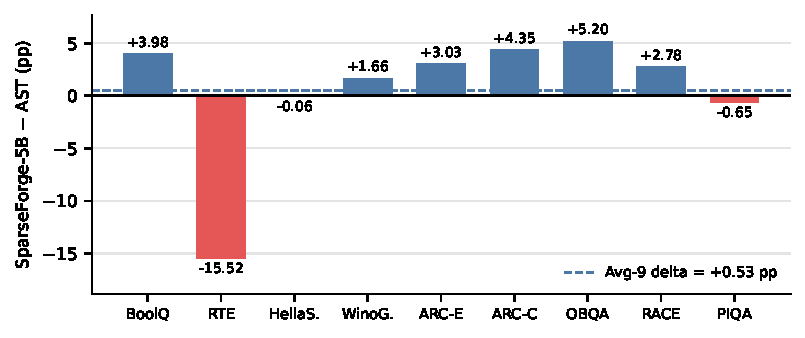
\includegraphics[width=0.85\columnwidth]{figures/checkpoint_delta.pdf}
  \caption{Per-task accuracy difference \method{}-5B minus the public AST deployable checkpoint under the same nine-task harness, computed from the harness CSV. The Avg-9 difference is $+0.53$ points (dashed line), but task-level behavior is strongly mixed: BoolQ, ARC-Easy, ARC-Challenge, OpenBookQA, and RACE contribute the gain, while RTE moves by $-15.52$ points. The aggregate advantage over the strongest $625$M fixed-support recovery endpoint is $+2.53$ points.}
  \label{fig:checkpoint}
\end{figure}

Table~\ref{tab:rte-audit} separates the earlier deviating RTE log from the
registered value and its denominator checks.  The anomaly is consistent with
a single-digit corruption (for example, a leading $4 \!\to\! 6$
substitution), while denominator back-solving verifies every per-task harness
cell against an integer example count.  We therefore use the registered RTE
value throughout.  It does not drive the recovery-compression result: the majority-share Avg-9
margin remains close enough to zero that a small task-level change can reverse
its sign.

\begin{table}[htbp]
\centering
\caption{RTE provenance and denominator checks for the 5B checkpoint.  The
earlier $69.82$ log is not representable as an integer correct count over 277
examples; the registered $49.82=138/277$ is used throughout.  The
$+0.528$-point Avg-9 margin remains sensitive to a small task-level change.}
\label{tab:rte-audit}
\small
\setlength{\tabcolsep}{5pt}
\begin{tabular}{@{}lp{0.16\textwidth}p{0.50\textwidth}@{}}
\toprule
Check & Value & Interpretation \\
\midrule
Earlier logged RTE cell & $69.82$ & No integer numerator over $n=277$ yields this percentage. \\
Registered RTE cell & $49.82$ & Exact at $138/277$; used in Table~\ref{tab:unified} and Figure~\ref{fig:checkpoint}. \\
RTE majority class & $52.71\%$ & Exact at $146/277$; neither RTE value is near this baseline, and the registered value is below chance. \\
Same-row WinoGrande & $69.85$ & Near-coincidence with the logged anomaly, consistent with a single-digit corruption. \\
Avg-9 margin & $+0.528$ pp & A change of $O(13)$ examples in one comparably weighted task can move it through zero. \\
\bottomrule
\end{tabular}
\end{table}

\paragraph{RTE diagnostic.}
The registered RTE result is $49.82\%$, below the $52.71\%$ majority-class
baseline; Table~\ref{tab:rte-audit} carries the provenance checks and the exact
integer counts behind both rates. Neither a label-order nor a prompt-template
ablation has been re-run in this workspace, so we cannot separate a harness
artifact from a recovery-side task regression, and the AST row of
Table~\ref{tab:unified} stays above chance on the same harness configuration.
The cause therefore remains unresolved and registered: we report the measured
cell without using it as evidence for or against the method, and its
leave-one-out consequence is isolated separately
(Appendix~\ref{app:stats}, Table~\ref{tab:loo}).

\subsection{What the Recovery Baselines Establish}
The narrow post-recovery spread among ALPS-, ELSA-, and ProxSparse-supported endpoints shows that joint sparse-weight/SLoRB healing improves several fixed supports while leaving an observable range far below the harness's per-checkpoint binomial-SE sampling-noise scale. It does not prove that one native support is universally best, nor that recovery makes the supports intrinsically equivalent. A longer-budget ELSA-support experiment failed under the tested QA-style recovery protocol after initially improving; this is evidence that the recipe requires redesign, not that ELSA generally fails at long budgets (Appendix~\ref{app:elsa-failure}, Figure~\ref{fig:elsa-recovery}).

\subsection{Archived Breadth and Deployment}
Archived single-run evaluations cover eight model families and are summarized in Appendix~\ref{app:archived}. They suggest broadly consistent but architecture-dependent transfer, so we keep the breadth claim out of the central result. Separately, archived H800 TensorRT-LLM measurements report $1.40$--$1.44\times$ throughput and $0.58\times$ weight memory for an export attributed to an earlier pipeline-generation checkpoint; these numbers do \emph{not} correspond to any export of the checkpoint evaluated in this paper (none exists), and their provenance---the identity of the exported checkpoint---is unverifiable in this workspace, so they are reporting-only historical records rather than a new systems benchmark.

\section{Limitations}\label{sec:limitations}
The load-bearing recovery-compression result uses three archived endpoints, not a contemporary multi-seed training study; the $0.52$\,pp quantity is a marginal per-checkpoint binomial-SE, not pairwise or joint uncertainty or training-run variance, and per-item predictions were not retained. Historical error bars in Appendix~\ref{app:history} use different legacy suites and cannot be transferred to the current harness. A valid matched-budget \method{} run at $625$M tokens is also missing, so the archived $5$B comparison is not a token-normalized sample-efficiency result. These three components have never been isolated under matched budgets; none of the reported gains can be attributed to any single mechanism. Equally critical: \textbf{no export exists}---every reported number is a branch-active training-state measurement; the SLoRB fold, exact $2{:}4$ re-projection, group-sum assertion, and pre/post-export quality are unimplemented/unmeasured (Appendix~\ref{app:implementation}, EXT-M3), so no deployment-equivalence or deployment-speed claim can be drawn from this paper's results. The resulting asset dependency is terminal within this study's scope: the fold checks and corpus disambiguation both require the archived weights and manifest, which are unreachable (Appendix~\ref{app:implementation}, archived-checkpoint unreachability disclosure), and this paper closes by reporting training-state measurements without fold or corpus claims. The curvature score, annealing schedule, and SLoRB branch are therefore pipeline background rather than title-level contributions. Curvature estimation and retraining cost more than one-shot pruning. Cross-family results are archived single runs without recoverable per-seed or full harness metadata, and Qwen-family degradation shows that recovery is architecture- and corpus-dependent. The failed long-budget ELSA-support recipe must be redesigned before drawing a method-level conclusion. Finally, deployment results cover one H800/TensorRT-LLM setup, so speedups may vary with hardware and workload.

\section{Conclusion}\label{sec:conclusion}
The transferable result is a descriptive endpoint observation bounded by the eval-sampling scale, not a mechanism victory: identical $625$M-token recovery compresses the registered cross-support \taskavg{} spread from $2.675$ to $0.118$\,pp, far below the per-checkpoint binomial-SE sampling-noise scale of this harness; whether they bear pairwise mechanism claims is unidentified without the paired per-item statistics this study did not register. The archived branch-active $5$B checkpoint remains supporting context; its corpus identity is unavailable, its component effects are not isolated, and its fold to a deployable exact-$2{:}4$ export is unmeasured future work. Matched-budget, multi-seed, and export measurements are therefore required before stronger method or deployment conclusions.

\paragraph{Ethical considerations.}
SparseForge uses an additional recovery corpus during post-training ($5$B tokens in the strong configuration; corpus provenance unavailable for the archived checkpoint, Appendix~\ref{app:implementation}); it does not add new capabilities to the dense model beyond adaptation to the same data distribution, but it does expose the compressed model to that recovery data. Compression may reduce inference memory and time but consumes recovery compute, and it inherits the base model's bias, privacy, licensing, and misuse risks. The reported measurements are not a life-cycle carbon assessment.

% P5_MAIN_TEXT_END
\label{p5:main-text-end}
\bibliographystyle{iclr2026_conference}
\bibliography{references,refs}

\appendix
% Keep compact appendix tables with their explanatory text without shrinking type.
\setlength{\intextsep}{6pt plus 2pt minus 2pt}
\setlength{\abovecaptionskip}{4pt}
\section{Statistical Appendix: Avg-9 Uncertainty and Recovery Compression}
\label{app:stats}
% Appendix B: significance of the SparseForge-vs-AST Avg-9 margin (binomial-SE, sign test)
% Appendix C: LOO-9 sensitivity and the 22x recovery-compression argument. Fragment authored by C5 (R138 P0-3, zero GPU); consumed verbatim.
% =====================================================================
% C5 zero-cost statistical block for S1 refine-1 Appendix B/C (R138) -- v2
% Author: C5. Input restricted to registered CSVs (CSV-CAST9, CSV-LWT).
% v2 changes vs v1: (1) formal 9-row Leave-One-Out table with Avg-8 margin
%   AND delta-vs-full columns (R138 P0-3 item 1); (2) per-task McNemar
%   explicitly annotated with the R138-required sentence
%     "McNemar omitted: per-item logs not available under R138 budget"
%   (R138 P0-3 item 2), replacing the previous prose-only boundary.
% Every number is reproducible from cast9_dense_ast_current_harness.csv
% with lm-eval standard dev-set sizes. Exact per-item McNemar is PROVABLY
% unidentifiable from the aggregate CSV (see Boundary). Compile as a
% fragment; S1 integrates into Appendix B/C.
% =====================================================================

\subsection{Sampling uncertainty of the archived SparseForge vs.\ AST margin}
\label{app:sf-ast-stats}

% r48/B3 layout-only: the unbreakable filename, numeric set, and task list forced
% four badness-10000 underfull lines here.  \allowbreak only adds legal break
% points; no character, number, or ordering changes.
% r49 layout-only follow-up: in the text-mode task list `\allowbreak RTE' also
% swallowed the inter-word space, so the parenthetical printed as
% "(BoolQ,RTE,HellaSwag,...)".  Ordinary spaces restore the words AND supply the
% glue that \allowbreak lacks, so they justify better than the penalty-only
% version did.  Same nine names, same order.
% r58 information-design fix (layout-only): the nine dev-set sizes were a
% 9-number wall inside this sentence.  They now sit in the new $n_k$ column of
% Table~\ref{tab:loo}, paired with the task each one belongs to; the values, the
% task order and the citation are unchanged.  The hardcoded "Table~1" is also
% replaced by \ref{tab:unified} so the cross-reference cannot silently rot.
We quantify the uncertainty of the archived comparison
$\mathrm{SparseForge}- \mathrm{AST}$ (Avg-9, Table~\ref{tab:unified}) using only
the registered same-harness per-task accuracies of
\texttt{cast9\_\allowbreak dense\_\allowbreak ast\_\allowbreak
current\_\allowbreak harness.csv} and the standard
lm-eval dev-set sizes $n_k$ of the nine tasks
(BoolQ, RTE, HellaSwag, WinoGrande, ARC-E, ARC-C, OBQA, RACE,
PIQA), which Table~\ref{tab:loo} lists task by task.

\paragraph{Leave-one-out (LOO-9).}
The full nine-task margin is
$\Delta_{\mathrm{Avg}{-}9}=+0.528$\,pp. Table~\ref{tab:loo} reports, for
each of the nine tasks dropped one at a time, the remaining eight-task
margin, $\Delta_{\mathrm{Avg}{-}8}^{(k)}$, and its deviation
$\delta_k=\Delta_{\mathrm{Avg}{-}8}^{(k)}-\Delta_{\mathrm{Avg}{-}9}$
from the full mean.

% r58 layout-only: caption moved above the tabular so that all seven tables use
% the same caption position (Tables 1, 3, 5, 6, 7 already did); the $n_k$ column
% absorbs the nine dev-set sizes that used to be a number wall in the paragraph
% above.  Every margin and deviation cell is byte-identical to the previous face.
\begin{table}[h]\centering\small\setlength{\tabcolsep}{5pt}
\caption{Leave-one-task-out sensitivity of the Avg-9 margin. $n_k$ is the
standard lm-eval dev-set size that enters the binomial standard errors.
Dropping the smallest task (OpenBookQA, $n{=}500$) reverses the sign of the
remaining eight-task margin to $-0.056$\,pp; dropping ARC-Challenge or BoolQ
collapses it to $\approx$0.05--0.10\,pp; only dropping the AST-side RTE deficit
(RTE $=$ SparseForge $49.82$ vs.\ AST $65.34$) inflates the margin to
$+2.535$\,pp ($\delta{=}{+}2.006$). The archived $+0.528$\,pp margin is not robust
to single-task removal.}
\label{tab:loo}
\begin{tabular}{lrcc}
\toprule
Dropped task & $n_k$ & $k$-drop Avg-8 margin (pp) & $\delta_k$ vs full (pp) \\
\midrule
OpenBookQA & $500$ & $-0.056$ & $-0.584$ \\
ARC-Challenge & $1{,}172$ & $+0.050$ & $-0.478$ \\
BoolQ & $3{,}270$ & $+0.097$ & $-0.431$ \\
ARC-Easy & $2{,}376$ & $+0.215$ & $-0.313$ \\
RACE & $1{,}045$ & $+0.247$ & $-0.281$ \\
WinoGrande & $1{,}267$ & $+0.387$ & $-0.141$ \\
HellaSwag & $10{,}042$ & $+0.602$ & $+0.074$ \\
PIQA & $1{,}838$ & $+0.676$ & $+0.148$ \\
RTE & $277$ & $+2.535$ & $+2.006$ \\
\bottomrule
\end{tabular}
\end{table}

\paragraph{Avg-9 sampling error.}
% r58 information-design fix (layout-only): the difference SE, z and p formed a
% third stacked comparable trio here; they now occupy the aggregate row of
% Table~\ref{tab:pertask-tests}.  No value was recomputed, rounded or dropped.
Treating each checkpoint as fixed and each task accuracy as binomial, the
sampling SE of an unweighted nine-task mean is
$\mathrm{SE}=(1/9)\sqrt{\smash{\sum_k p_k(1-p_k)/n_k}}$, giving
$\mathrm{SE}_\mathrm{SF}=0.52$\,pp and $\mathrm{SE}_\mathrm{AST}=0.51$\,pp
per checkpoint. The resulting difference SE and the $z$ and two-sided $p$ of the
archived margin are the aggregate row of Table~\ref{tab:pertask-tests}: the
observed margin lies inside sampling noise.

\paragraph{Per-task tests.}
\textbf{McNemar omitted: per-item logs are not available in the registered artifacts.}
Exact per-example McNemar would require the discordant-pair counts
$b=\#(\mathrm{SF}\,\text{right},\mathrm{AST}\,\text{wrong})$ and
$c=\#(\mathrm{SF}\,\text{wrong},\mathrm{AST}\,\text{right})$ per task;
these are provably \emph{unidentifiable} from the registered aggregate
CSV, which records only the marginal correct counts
(SF\_correct$=a+b$, AST\_correct$=a+c$; only $b-c$ is fixed, and infinitely
many $(a,b,c,d)$ decompositions meet both margins). Per-item predictions for
these nine tasks are not available in the registered artifacts. The
strongest test computable from the registered data is therefore the unpaired
normal-approximation $z$-test on the difference of two independent binomial
proportions (equal $n$ in both arms). Table~\ref{tab:pertask-tests} collects
every test statistic that the registered data support. At the uncorrected 5\%
level, four tasks are significant (BoolQ, RTE, ARC-Easy, ARC-Challenge); under
Holm correction across nine tasks, only BoolQ and RTE remain significant.

% r65 W1 (R223): full nine-task SE/z/p computed from the registered aggregate
% CSV in the same two-proportion convention; previously reported z values
% cross-checked (BoolQ +3.79, RTE -3.70, OBQA +1.75, pooled +2.63) and match.
% No per-item logs exist, so none of these is a paired test.
\begin{table}[h]\centering\small\setlength{\tabcolsep}{3.2pt}
\caption{Significance tests computable from the registered aggregate CSV;
$\Delta$ is SparseForge $-$ AST. All per-task rows use the same unpooled
two-proportion $z$ convention (equal $n$ in both arms); SE is the sampling
SE of the accuracy difference. No per-item logs exist, so none of these is a
paired test. Under the uncorrected 5\% convention four task-level pairs
reach significance (BoolQ, RTE, ARC-Easy, ARC-Challenge); under Holm
correction across the nine tasks only BoolQ and RTE do. The pooled
count-level row and the Avg-9 row are reported as in the earlier revision.
The final column reports uncorrected/Holm significance.}
\label{tab:pertask-tests}
\begin{tabular}{@{}lrrrrrc@{}}
\toprule
Comparison (test) & $\Delta$ & SE & $z$ & $p$ & $p_{\rm Holm}$ & Sig. raw/Holm \\
\midrule
BoolQ & $+3.97$ & $1.05$ & ${+}3.79$ & $0.0002$ & $0.0013$ & yes/yes \\
RTE & $-15.52$ & $4.20$ & ${-}3.70$ & $0.0002$ & $0.0015$ & yes/yes \\
HellaSwag & $-0.06$ & $0.70$ & ${-}0.08$ & $0.932$ & $1.0000$ & no/no \\
WinoGrande & $+1.66$ & $1.84$ & ${+}0.90$ & $0.367$ & $1.0000$ & no/no \\
ARC-Easy & $+3.03$ & $1.26$ & ${+}2.41$ & $0.016$ & $0.1118$ & yes/no \\
ARC-Challenge & $+4.35$ & $2.04$ & ${+}2.14$ & $0.033$ & $0.1948$ & yes/no \\
OpenBookQA & $+5.20$ & $2.97$ & ${+}1.75$ & $0.079$ & $0.3948$ & no/no \\
RACE & $+2.78$ & $2.15$ & ${+}1.29$ & $0.196$ & $0.7825$ & no/no \\
PIQA & $-0.66$ & $1.40$ & ${-}0.47$ & $0.640$ & $1.0000$ & no/no \\
\midrule
Nine tasks (pooled count $z$) & $+1.23$ & $0.47$ & ${+}2.63$ & $0.008$ & -- & -- \\
Nine tasks (6/9 wins, exact sign) & --- & --- & --- & $0.508$ & -- & -- \\
\taskavg{} margin (checkpoint $z$) & $+0.528$ & $0.73$ & ${+}0.72$ & $0.47$ & -- & -- \\
\bottomrule
\end{tabular}
\end{table}

\paragraph{Boundary.}
A per-example paired (McNemar) analysis would be the decisive tighter test,
but it requires per-item predictions that are not in the registered set
in the registered artifacts; it is gated on a future registered run
producing per-item inference outputs, and is not computable from the
aggregate CSV. This boundary is stated verbatim in the machine-readable
delivery (\texttt{stat\_delivery\_v2.json}).

\subsection{Recovery compresses the cross-support spread below the sampling-noise scale}
\label{app:recovery-compression}

% r58 information-design fix: this table's only cross-reference was inside
% the descriptive implication paragraph; the introducing sentence names it in
% running prose as well.  Wording otherwise unchanged.
Table~\ref{tab:recovery-compression} reports native and identical 625M-token joint
weight+SLoRB recovery results from
\texttt{trainingfree\_lowtraining\_detailed\_ast7.csv}. The post-recovery range
$R(T)=0.118$\,pp is far below the $0.52$\,pp per-checkpoint binomial-SE
sampling-noise scale\footnote{The $0.52$\,pp term is the per-checkpoint \taskavg{} binomial-SE; pairwise and joint (max-min) uncertainty involve covariance and selection effects not captured by a single marginal SE, and require per-item predictions not contained in the registered aggregate CSVs}. Its joint uncertainty is unidentified from the registered aggregates, so we do not quote a compression ratio.

% r58 layout-only: caption moved above the tabular for consistency with the other
% six tables.  Cells unchanged.
\begin{table}[h]\centering\small\setlength{\tabcolsep}{6pt}
\caption{Recovery compresses the cross-support range from 2.675\,pp to
0.118\,pp, far below the $0.52$\,pp per-checkpoint binomial-SE sampling-noise
scale (\S\ref{app:sf-ast-stats}). This is a descriptive marginal-scale comparison;
the aggregates do not identify paired or joint uncertainty. The weaker native
supports gain most and the ALPS$\leftrightarrow$ProxSparse rank flips.}
\label{tab:recovery-compression}
\begin{tabular}{lccc}
\toprule
Support & native AVG-9 (0 tok) & recovered AVG-9 (625M) & gain \\
\midrule
ALPS & 52.12 & 55.82 & $+3.70$ \\
ELSA-4096 & 54.59 & 55.94 & $+1.34$ \\
ProxSparse & 51.92 & 55.91 & $+3.99$ \\
\midrule
range & 2.675 & 0.118 & \\
\bottomrule
\end{tabular}
\end{table}

\paragraph{Conjecture (C1): annealed-support signal survives compression only via an asymptotic intercept.}
\label{conj:survival}
The following is a \emph{conjectured} regime statement, not a proved theorem: it is displayed because an
external soundness review exhibited an explicit counterexample to the corresponding unconditioned claim
(one can place the observed range $R(T)$ into the recovery-invariant subspace while keeping the
transients active, so the ``iff'' fails at finite $T$), and\emph{no} stronger bounded-$T$ claim is made
in this revision. We state the conjectured repair so the reader sees our best current mechanism
explanation and the assumptions that would have to hold for it to be adequate.
Let $A_s(0)$ and $A_s(T)$ be the AVG-9 of support $s$ before and after
$T$ recovery tokens, and let $\phi_s = \lim_{T\to\infty} A_s(T)$ be the
recovery attractor; assume the intercepts exist (conjectured regime, not established).
Suppose
$A_s(T) = \phi_s + \bigl(A_s(0)-\phi_s\bigr)\,g_s(T)$ with $g_s(T)\to0$ in a recovery-dominated regime
($T$ large enough that the transient term is uniformly dominated).
Then the cross-support range
$R(T)=\max_s A_s(T)-\min_s A_s(T)$ converges to
$\lim_{T\to\infty}R(T)=\max_s\phi_s-\min_s\phi_s$.
If the supports share one attractor ($\phi_s=\phi_{s'}$ for all $s,s'$), then
for any $T$ with $g_s(T)\approx g_{s'}(T)$ the native signal is erased:
$A_s(T)-A_{s'}(T)\approx0$ up to recovery noise, and rank orders that depend
only on the transient $A_s(0)-\phi_s$ are not recoverable. Under the conjectured regime above
(regime rate condition: the transient $g_s(T)$ contribution is dominated by the intercept
contribution to $R(T)$) we \emph{conjecture}
that a support/mask signal survives recovery-compression iff
it is carried by an \emph{asymptotic intercept}
$\phi_s-\phi_{s'}\neq0$ that (i) is monotone under the recovery-preserving
transformation and (ii) is not absorbed into a shared fixed point, i.e.\ the
advantage lies in the recovery-invariant subspace. The two-line calculation that
$R(T)\to\max_s\phi_s-\min_s\phi_s$ is the only step we can justify in this revision.
The existence and joint uncertainty of distinct intercepts relative to the $0.52$\,pp
per-checkpoint binomial-SE sampling-noise scale, and the recovery-invariant-subspace
statement, remain open.

\paragraph{Implication (descriptive).}
SparseForge's $+0.53$\,pp over AST uses $5$B recovery tokens, an $8\times$ larger
budget than the $625$M rows in~Table~\ref{tab:recovery-compression}, where the
cross-support range is far below the $0.52$\,pp binomial-SE sampling-noise scale.
Because the conjectured regime conditions and paired/joint uncertainty are unverified,
we draw no conclusion beyond budget confounding. No registered
experiment measures SparseForge's own support at 625M (the resolving row), so
the $+0.53$\,pp claim remains budget-confounded and is not yet attributable
to the mask mechanism.

\section{ELSA Fixed-Support Long-Budget Failure Mode}
\label{app:elsa-failure}
Figure~\ref{fig:elsa-recovery} shows that the longer-budget ELSA-support curve improves, then destabilizes, then diverges; its caption carries the registered per-step values. This is the only on-disk experiment with complete per-run raw artifacts; its divergence (not a mechanism-level failure of ELSA as a method) is why Sec.~\ref{sec:limitations} frames the failure as ``the longer-budget recipe requires redesign, not that ELSA generally fails.''

% Keep the deferred failure curve before Appendix C without stretching the
% shorter figure page's section spacing; normal flush-bottom layout resumes
% after the following unbreakable protocol table and its footnote.
\raggedbottom
\begin{figure}[H]
  \centering
  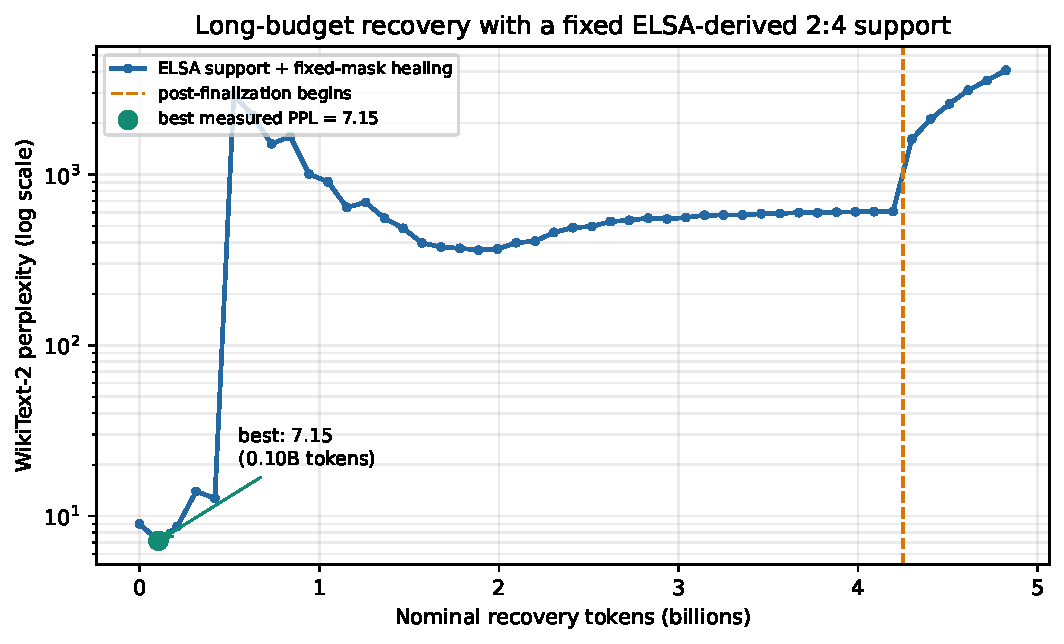
\includegraphics[width=0.9\columnwidth]{figures/elsa_fixed_support_sf5b_recovery_curve.pdf}
  \caption{Registered recovery trajectory of the fixed ELSA support on the
  $5$B-token \method{} recovery stream: PPL drops from $8.99$ (step $0$) to a minimum of $7.15$ (step $100$), destabilizes step $300 \to 500$, and diverges past step $1000$ ($2930$ at step $500$, $4083$ at step $4600$). Raw per-step values are included in the anonymous artifact.}
  \label{fig:elsa-recovery}
\end{figure}

\begin{samepage}
\section{Implementation Details and Artifact Statement}
\label{app:implementation}

% r69 P0-2 provenance, frozen source only (commit 520170b91757312f0aeef16b4b899fc3397963a4):
% legacy/sparse_modeling.py:136-239 (configuration and tensor semantics),
% legacy/main_llama.py:125-175 (optimizer betas and rank-offset seeding), and
% experiments/rebuttal_2026/scripts/archive_run_fixed_mask_sparseforge_5b_aligned.sh:25-41,67-90,128-205.
This appendix is the executable specification of the learned-mask path at the
frozen code commit
\texttt{520170b9}. It separates that algorithm
from the archived fixed-support recovery launchers: the latter set
\texttt{change\_mask=False}, so their mask, temperature, structural-mixing,
and hardening schedules are inactive. Table~\ref{tab:hyperparams} collects the operating
constants of those reported recovery arms; the paragraphs after the table
specify the active learned-mask algorithm and its export boundary.
\end{samepage}

\begin{table}[H]
\centering\small
\caption{Hyperparameters and protocol constants of the reported SparseForge
recovery arms. ``625M'' rows are the three fixed-support recovery endpoints;
``5B'' is the single archived configuration used as supporting context. A dash marks a
quantity not fixed by the archived run protocol. Unspanned rows give the two
arms separately in the two value columns; a value spanning both columns applies
to the 625M recovery arm and the 5B strong configuration alike.}
\label{tab:hyperparams}
\setlength{\tabcolsep}{5pt}
\begin{tabular}{@{}lll@{}}
\toprule
Quantity & 625M recovery rows & 5B strong configuration \\
\midrule
Optimizer & custom AdamW & custom AdamW \\
Adam betas & \multicolumn{2}{c}{$\beta_1{=}0.9,\ \beta_2{=}0.95$} \\
Fused optimizer kernel & no & no \\
Base random seed & 0 & 0 \\
Sequence length & 2048 & 4096 \\
Global batch size (seq) & 256 & 256 \\
Micro batch size & 1 & 8 \\
Total steps & 1192 & 4768 ($=4053{+}715$) \\
Peak step size & $2\times10^{-5}$ & $1\times10^{-4}$ \\
Final step size & $2\times10^{-6}$ & $1\times10^{-5}$ \\
Step-decay schedule & cosine & cosine \\
Warmup steps & 50 & 477 \\
Step-weight decay & 0 & 0.1 \\
$\lambda_{\rm KL}:\lambda_{\rm task}$ & \multicolumn{2}{c}{$1{:}1$ (CE + KL)} \\
KL teacher & \multicolumn{2}{c}{the pre-finetune dense checkpoint itself} \\
Distillation temperature & 2.0 & code default\footnotemark \\
Mask-temperature $T$ (initial) & 0.7 (launcher record) & 1.0 (code default; manifest records no override\footnotemark) \\
SLoRB rank / init & \multicolumn{2}{c}{$16$ / zero-init} \\
Hardening start (step) & inactive & 2861 \\
Hardening duration (steps) & inactive & 1192 \\
Mask-switch step & 477 & 477 \\
Post-finalization finetune & disabled & 715 \\
Transformers & \multicolumn{2}{c}{\texttt{4.57.6}} \\
lm-eval-harness & \multicolumn{2}{c}{$\geq0.4.0$} \\
\bottomrule
\end{tabular}
\end{table}
\footnotetext{The portable 625M launcher pins a distillation temperature of
2.0. The archived 5B launch manifest does not record a temperature override,
so the trainer's code default applies. We report this distinction explicitly
rather than silently substitute one default for the other. The frozen LLaMA
path imports the repository-local \texttt{legacy/adamw.py}; it does not pass a
\texttt{fused} flag or dispatch to PyTorch's fused AdamW kernel.}
\footnotetext{The archived 5B launch manifest records no mask-temperature
override, so the trainer's code default 1.0 applies on the 5B side; the 0.7
record in the portable 625M launcher is reported literally to its left.}
\flushbottom

% r69 P0-2 provenance: legacy/sparse_modeling.py:242-405,720-825;
% legacy/main_llama.py:2109-2230,2279-2330 (all line numbers at commit 520170b9).
\subsection{Executable alternating weight/mask algorithm}
For every sparse linear layer $\ell$, let
$W_\ell,m_\ell,H_\ell\in\mathbb{R}^{d_{\mathrm{out}}\times
d_{\mathrm{in}}}$, with $d_{\mathrm{in}}$ divisible by $M=4$. The code views
each row as $d_{\mathrm{in}}/4$ consecutive groups, hence grouped tensors have
shape $d_{\mathrm{out}}\times(d_{\mathrm{in}}/4)\times4$, and retains
$N=2$ indices in the final hard mask. The SLoRB forward branch is
$B_\ell P_\ell$, implemented as two linear maps after the masked base-weight
map; $P_\ell$ is fixed unless \texttt{trainable\_projection=True}.

% MINOR-9 fix (r72 full-fix): the block must not split silently, but as ONE
% minipage it no longer fitted after Table~\ref{tab:hyperparams} and pushed
% ~16 blank lines to the bottom of the preceding page.  Two atomic parts with an
% explicit "(continued)" heading remove both the silent split and the whitespace
% hole; step numbering continues through \setcounter{enumi}.  Both the content
% and the closing rule sit at the same \linewidth inside \begin{quote}, so the
% rule cannot exceed the text block (BLOCKER-1) and is left-aligned with the
% steps.
\begin{minipage}{\linewidth}
\paragraph{Algorithm 1: alternating weight and mask tracks.}
\begin{quote}\small
\textbf{Input:} training batches; $W_\ell$; continuous masks
$m_\ell\in[0,1]^{d_{\mathrm{out}}\times d_{\mathrm{in}}}$; SLoRB factors
$(B_\ell,P_\ell)$; update period $K$; and schedules below.
\begin{enumerate}
  \item For optimizer step $t$ and each gradient-accumulation micro-step,
  compute each sparse-linear output with $m_{\mathrm{eff},\ell}$ and the SLoRB
  add-on, then form
  $\mathcal{L}_{\mathrm{train}}=\lambda_{\mathrm{task}}\mathrm{CE}
  +\lambda_{\mathrm{KL}}\mathrm{KL}$ (both coefficients are $1$ in the
  reported distillation recipe).
  \item On the last micro-step only, if \texttt{enable\_hutchinson=True}, draw
  one independent Rademacher tensor per $W_\ell$ and update $H_\ell$ by the
  double-backward rule in the next subsection. The differentiated parameter
  list contains the sparse base weights $W_\ell$ only, not masks or SLoRB
  factors.
  \item Back-propagate the accumulated loss and take one AdamW weight-track
  step on the trainable parameters. The mask is a non-autograd parameter and
  is not changed by this optimizer step.
\end{enumerate}
\end{quote}
\end{minipage}

\begin{minipage}{\linewidth}
\paragraph{Algorithm 1 (continued): mask track and finalization.}
\begin{quote}\small
\begin{enumerate}
  \setcounter{enumi}{3}
  \item If $t$ is before \texttt{sparsity\_warmup\_steps}, or $t\bmod K\ne0$,
  skip the mask track. Otherwise, using the post-optimizer $W_\ell$, compute
  the standardized Hessian--OBD scores, groupwise gate and exact top-$2$
  target, structural mixture, $2{:}4$ penalty pull, and mask EMA specified
  below. Update the stored hardening coefficient $h_x$ on this same mask
  update.
  \item After the final step, construct the hard top-$2$ mask, apply the
  implemented state-dict finalization, run the exact support assertion below
  (per-group sum $=2$; specified as the required export unit check but not
  wired into the frozen validator, Appendix~\ref{app:implementation}),
  and save the checkpoint. The distinct SLoRB-fold/re-projection operation is
  not implemented by this finalizer and is therefore a separate future export
  measurement, not an executed line of Algorithm~1.
\end{enumerate}
\noindent\rule{\linewidth}{0.4pt}
\end{quote}
\end{minipage}

% r69 P0-2 provenance: legacy/utils.py:710-868; legacy/main_llama.py:2109-2230.
\subsection{Hutchinson diagonal on the training loss}
On the last micro-step of every enabled optimizer update, the implementation
passes the (gradient-accumulation-scaled) training loss to
\texttt{update\_hessian\_hutchinson}. Terms depending only on the detached
mask do not alter its derivatives with respect to $W$. For every sparse base
weight and one fresh probe $v_\ell\sim\mathrm{Rad}(\{-1,+1\})^{W_\ell}$, it
computes
\begin{equation}
g_\ell=\nabla_{W_\ell}\mathcal{L}_{\mathrm{train}},\qquad
u=\sum_\ell\langle g_\ell,v_\ell\rangle,\qquad
\widehat H_\ell=\max\!\left(0,
  \nabla_{W_\ell}u\odot v_\ell\right).
\end{equation}
The first \texttt{torch.autograd.grad} uses
\texttt{create\_graph=True}; the second differentiates $u$ with respect to
the same $W$-only list. Thus this is one Hutchinson sample per enabled update,
not one sample per mask update and not an average over accumulation
micro-steps. In DDP, $\widehat H_\ell$ is all-reduced and divided by the world
size before the EMA
$H_\ell\leftarrow0.99H_\ell+0.01\widehat H_\ell$; $0.99$ is
\texttt{cfg.beta}. The frozen FSDP branch instead updates local shards without
that DDP all-reduce, a distinction required to reproduce the code exactly.

% r69 P0-2 provenance: legacy/sparse_modeling.py:1020-1242 (score/gate),
% 935-988 (temperature and beta schedules), and 1167-1188 (structured_exact).
\subsection{Score, gate, schedules, and mask recurrence}
The \texttt{hessian\_obd} metric forms
$S^{\mathrm{raw}}_\ell=(H_\ell+10^{-8})\odot W_\ell^2$ and standardizes it
over the complete layer,
\begin{equation}
S_\ell=\frac{S^{\mathrm{raw}}_\ell-\mu(S^{\mathrm{raw}}_\ell)}
 {\operatorname{std}(S^{\mathrm{raw}}_\ell)+10^{-6}}.
\end{equation}
After reshaping to
$d_{\mathrm{out}}\times(d_{\mathrm{in}}/4)\times4$, let $I_g$ be the two
indices returned by \texttt{torch.topk} and let $\bar G_g$ be zeros with ones
scattered at $I_g$. In the soft structured path, the implemented threshold is
the second-largest score $\tau_g=S_{g,(2)}$ (not the midpoint of the second-
and third-largest scores), and
$G^{\mathrm{soft}}_g=\sigma((S_g-\tau_g)/(T+10^{-8}))$.
If \texttt{structured\_exact=True}, the code bypasses this sigmoid and returns
$\bar G_g$ directly.

With $K=\texttt{mask\_update\_period}=10$, the default temperature schedule is
\begin{equation}
T(t)=\max\!\left(0.05,\;1.0\times0.97^{\lfloor t/K\rfloor}\right),
\end{equation}
corresponding to \texttt{temp\_init=1.0}, \texttt{temp\_min=0.05}, and
\texttt{temp\_decay=0.97}. Mask updates occur only when
$t\ge\texttt{sparsity\_warmup\_steps}$ and $t\bmod K=0$. For configured
structural endpoints $t_s<t_e$, set
$q=\operatorname{clip}((t-t_s)/(t_e-t_s),0,1)$ and
$\beta(t)=3q^2-2q^3$; then
$G^\beta=(1-\beta)G^{\mathrm{soft}}+\beta\bar G$. A disabled interval
($t_e\le t_s$) yields $\beta=0$.

% r69 P0-2 provenance: legacy/sparse_modeling.py:1246-1622, especially
% 1284-1299,1353-1396,1595-1622; legacy/main_llama.py:2163-2177.
For \texttt{mask\_penalty\_mode=nm\_2\_4}, the code takes another per-group
top-$2$ target $\bar G^{m}$ from the current gate ordering and applies the
no-grad pull
\begin{equation}
\begin{aligned}
G' & = \operatorname{clip}_{[0,1]}\!\left[
G^\beta-(\texttt{pen\_scale}\,\lambda_{\mathrm{mid}})
(m-\bar G^{m})\right],\\
m & \leftarrow(1-a)m+aG',\qquad a=\texttt{mask\_lr}=0.10.
\end{aligned}
\end{equation}
Here \texttt{pen\_scale} is \texttt{mask\_penalty\_lr}, falling back to
\texttt{mask\_lr} when unset; in the non-block modes
$\lambda_{\mathrm{mid}}$ ramps linearly from zero to its configured maximum
over the first 500 optimizer steps and then remains constant.

% r69 P0-2 provenance: legacy/sparse_modeling.py:720-825 and 1606-1622.
For hardening start $t_h$ and duration $D$, the stored coefficient is
$h_x=1$ before $t_h$, $h_x=1-(t-t_h)/D$ on the interval, and $h_x=0$ at and
after $t_h+D$ (clipped to $[0,1]$ and refreshed on mask-update steps). The
forward pass uses
\begin{equation}
m_{\mathrm{eff}}=h_xm+(1-h_x)\bar G^m.
\end{equation}
If CAST-style \texttt{weight\_scaling} is enabled, its $2{:}4$ target factor
is $M/N=2$ and the actually applied factor is
$c(h_x)=1+(1-h_x)(2-1)$; it therefore anneals from $1$ to $2$ with the same
$h_x$. The reported fixed-support launcher disables this option.

% r69 P0-2 provenance: legacy/sparse_modeling.py:1167-1188 and 1210-1228;
% legacy/main_llama.py:2734-2750 at commit 520170b9.
\subsection{Tie rule and exact-$2{:}4$ validation}
Every structured selection uses the indices returned by
\texttt{torch.topk(..., largest=True)} and creates the binary target by
\texttt{scatter\_}. This guarantees two written ones per group for a returned
index tuple, including the \texttt{structured\_exact} path, but the frozen
code adds no deterministic secondary key. PyTorch/CUDA does not expose a
stable mathematical ordering for equal scores, so tied groups have an
underspecified support: the kernel's returned indices decide the survivors,
and a unique cross-device tie rule is not guaranteed.

The required export unit assertion is therefore the groupwise, not merely
global, check
\begin{verbatim}
assert torch.all(hard.view(d_out,d_in//4,4).sum(-1) == 2)
\end{verbatim}
At the frozen commit, \texttt{legacy/check\_sparsity.py:57--121,137--181}
checks binary/global mask sparsity and mask--weight zero overlap, but contains
\emph{no} group-sum-$=2$ assertion. It cannot honestly be cited as that exact
unit test until the assertion above is added to the export validator. During
training, \texttt{nm\_2\_4\_tile\_stats}
(\texttt{legacy/utils.py:1029--1234}) reports top-$2$/bottom-$2$ mask means and
soft--hard gaps; these are useful trajectory diagnostics but do not replace
the exact export assertion.

% r69 P0-2 provenance: legacy/sparse_modeling.py:790-875 (SLoRB forward/factors);
% legacy/main_llama.py:2649-2834 (state-dict hardening/apply/save) at commit 520170b9.
\subsection{Finalization, SLoRB fold boundary, and EXT-M3}
The algebraic fold needed to remove the inference branch would first form
$W^{\mathrm{fold}}_\ell=W_\ell+B_\ell P_\ell$ and then re-project
$W^{\mathrm{export}}_\ell=\Pi_{2{:}4}(W^{\mathrm{fold}}_\ell)$. The frozen
\texttt{main\_llama.py} finalizer does less: it recomputes a hard mask from
the soft mask, writes that mask to the state dict, replaces
$W_\ell$ by $W_\ell\odot\bar G_\ell$, and saves \texttt{model.pt}. It does
not add $B_\ell P_\ell$ into $W_\ell$ in this path. Consequently, neither the
fold-then-$2{:}4$ re-projection delta nor pre/post-export WikiText-2 PPL,
\taskavg{}, or support-change has been measured. We register those four
checks as future measurement \textbf{EXT-M3}; no deployment-equivalence claim
is inferred from the training checkpoint.

% r69 P0-2 provenance: legacy/main_llama.py:125-175 and 993-1016;
% legacy/model_llama.py:151-160; legacy/adamw.py:9-176; requirements.txt:1-21.
\subsection{Optimizer and software environment}
The frozen LLaMA path uses the repository-local AdamW implementation with
$\beta_1=0.9$, $\beta_2=0.95$, weight decay $0.1$ on matrix parameters and
zero decay on lower-dimensional parameters. The archived launch manifest pins
base seed $0$; DDP adds the rank to that seed. This optimizer is Python/tensor
AdamW rather than a fused optimizer kernel. The committed environment contract
pins \texttt{transformers==4.57.6} and requires
\texttt{lm\_eval>=0.4.0}; the latter is a lower bound rather than an exact
version, so a bitwise reproduction must additionally record the resolved
environment.

\textbf{Artifact statement.} The training entry point is the repository's
legacy \texttt{main\_llama.py}; fixed-support launchers are included in the
anonymous artifact. Evaluation uses
lm-evaluation-harness in the local wrapper
\texttt{eval\_\allowbreak native\_\allowbreak checkpoint\_\allowbreak shard.py}.
The recovery corpus of the archived 5B checkpoint is not named in this paper:
that corpus is recorded in a training manifest (\texttt{args.json}) archived
with the checkpoint on an archive host unreachable from this workspace since
2026-08-16, so the identity of the archived recovery corpus cannot be verified
from available materials. The modern matched-budget controls under preparation
(Appendix~\ref{app:stats}, Table~\ref{tab:unified} caption) use the locally
tokenized Dolmino-mix-1124 stream instead. The identifying repository URL is
replaced for double-blind review by the anonymized mirror
\url{https://anonymous.4open.science/r/SparseForge-Anonymous/}.

\subsection{Archived-checkpoint unreachability disclosure}
\label{app:r243closure}
The 5B headline checkpoint, its training manifest (\texttt{args.json}), and
its recovery-corpus tokenization live on an archive host that is unreachable
from this workspace;
independent re-scans of local storage returned no copy. Consequently: (i) the
archived recovery corpus is not named anywhere in this paper --- earlier
revisions' conflicting attributions (a Dolmino-style mix in the setup
paragraph; a QA-format SFT configuration in the artifact statement) cannot be
disambiguated from available materials and have been withdrawn; (ii)
fold/re-projection would require the archived branch parameters and is
registered as future measurement (EXT-M3); and (iii) every reported \method{}
number in this paper remains a branch-active training-state measurement whose
corpus provenance and export correspondence are unresolved. We disclose, and
the record does not allow us to resolve either dependency from the materials at
hand.

\section{Archived Cross-Family Evidence}
\label{app:archived}
Table~\ref{tab:archived} preserves archived single-run block-16 results as
model-family breadth evidence only.
\begin{table}[H]
\centering
% r58 information-design fix: this caption was purely descriptive and carried no
% takeaway.  The added clause restates the claims the paper already makes in
% Sec.~5.4 ("broadly consistent but architecture-dependent transfer"), in
% Limitations ("Qwen-family degradation") and in the paragraph above; no new
% comparison, number or claim is introduced.
\caption{Archived single-run block-16 mean accuracy. A registered-pack grep
found no headline-value hits, so the unrecoverable seven-task suite is not
named. All rows are English-only;
the axis is model family, not language. Diff is sparse minus dense. Transfer is
broadly consistent but architecture-dependent, with Qwen3-1.7B the largest
degradation; these are breadth records, not a controlled cross-family claim.}
\label{tab:archived}
\small
\begin{tabular}{lrrr}
\toprule
Model & Dense & Sparse & Diff \\
\midrule
LLaMA-2-7B & 59.70 & 59.02 & $-0.68$ \\
OPT-2.7B & 47.76 & 47.93 & $+0.17$ \\
GPT-2 & 37.13 & 37.58 & $+0.45$ \\
GPT-2-Medium & 41.01 & 39.45 & $-1.56$ \\
GPT-2-Large & 42.65 & 41.87 & $-0.81$ \\
GPT-2-XL & 45.49 & 45.14 & $-0.35$ \\
Qwen3-1.7B & 56.47 & 53.49 & $-2.98$ \\
DeepSeek-MoE-16B & 59.54 & 58.20 & $-1.34$ \\
\bottomrule
\end{tabular}
\end{table}

\section{Historical Training-Run Variability}
\label{app:history}
Table~\ref{tab:historical} preserves author-confirmed three-run aggregates;
missing run mappings and different legacy suites make the rows mutually and
currently incomparable.
\begin{table}[H]
\centering
% r58 information-design fix: takeaway added by restating the non-comparability
% caveat already stated in the paragraph above and in Limitations.
\caption{Historical three-run aggregates (mean $\pm$ sample SD). Corpus labels
are unverified contemporaneous records; because the rows use different legacy
suites, neither is comparable with the other or the current harness.}
\label{tab:historical}
\small
\begin{tabular}{llrr}
\toprule
Setting & Legacy suite & Accuracy & Wiki PPL \\
\midrule
5B Dolmino & CAST-7 & $57.27\pm0.09$ & $6.22\pm0.04$ \\
1.25B C4 & AST-7 & $57.23\pm0.13$ & $6.38\pm0.03$ \\
\bottomrule
\end{tabular}
\end{table}

\section{Baseline Dispersion}
\label{app:dispersion}
Table~\ref{tab:dispersion} reports sample SDs from three independent baseline
seeds where available (accuracy to two decimals, PPL to four); Table~\ref{tab:unified}
gives the means.
\begin{table}[H]
\centering
\caption{Three-seed sample SD under the unified harness. Aggregate SD appears
only for paired per-seed aggregates; a dash means it is not inferred from
marginal task statistics.}
\label{tab:dispersion}
\setlength{\tabcolsep}{2.4pt}
% r48/B3 layout-only: this last appendix page is over half empty, so \scriptsize
% was needless shrinkage; \small keeps the same columns within \textwidth.
\small
\begin{tabular*}{\textwidth}{@{\extracolsep{\fill}}lrrrrrrrrrrr}
\toprule
Method & BQ & RTE & Hella. & Wino. & ARC-e & ARC-c & OBQA & RACE & PIQA & \taskavg & PPL \\
\midrule
Wanda & 0.14 & 0.36 & 0.12 & 0.08 & 0.49 & 0.48 & 0.31 & 0.15 & 0.26 & 0.13 & 0.0525 \\
SparseGPT & 1.29 & 1.65 & 0.09 & 0.72 & 0.86 & 0.26 & 0.92 & 0.19 & 0.25 & 0.36 & 0.0103 \\
ALPS & 1.34 & 0.36 & 0.18 & 0.28 & 0.68 & 0.85 & 0.70 & 0.64 & 0.24 & -- & 0.0896 \\
ELSA (4,096 steps) & 1.06 & 2.54 & 0.06 & 0.83 & 0.56 & 0.53 & 0.64 & 1.23 & 0.17 & -- & 0.0168 \\
\bottomrule
\end{tabular*}
\end{table}

\end{document}
